\mcmSection{模型的建立与求解}

\mcmSubsection{问题一:分析数据得到客流函数}

近年来,笔者居住地政府并未公布有关地铁单日内分钟级或小时级的客流量数据,因此以深圳市政府数据开放平台曾公布的深圳通刷卡数据为数据来源。使用 Python 对数据进行流式处理,清洗无效数据、去除不需要的字段,保存到每个站点分别一个 TXT 文件,并对时间排序。设此原始数据为 $E_i(t)$。

\begin{figure}[htbp]
    \centering
    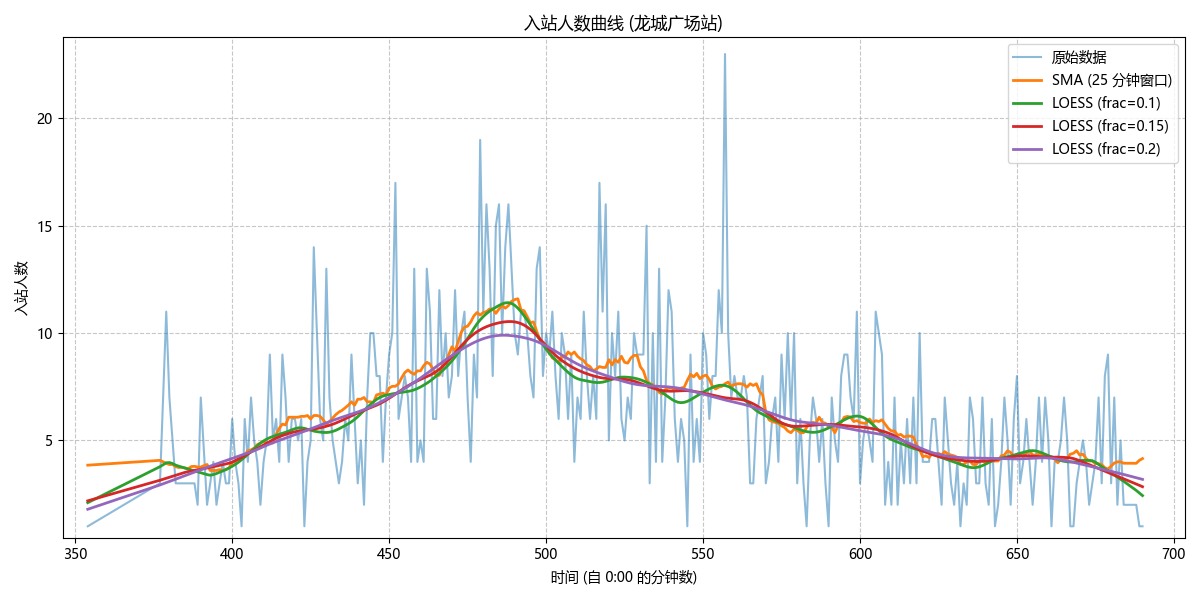
\includegraphics[width=1.0\textwidth]{res/Figure_1.png}
    \label{fig:entryCurveLongcheng}
\end{figure}

原始数据 $E_i(t)$ 存在显著的随机波动。为了提取潜在的客流模式,我们首先采用局部加权散点平滑(LOESS)\cite{1979LOESS}\cite{1988LOESS}技术,如图(以龙城广场站为例) \ref{fig:entryCurveLongcheng} 所示

\begin{figure}[htbp]
    \centering
    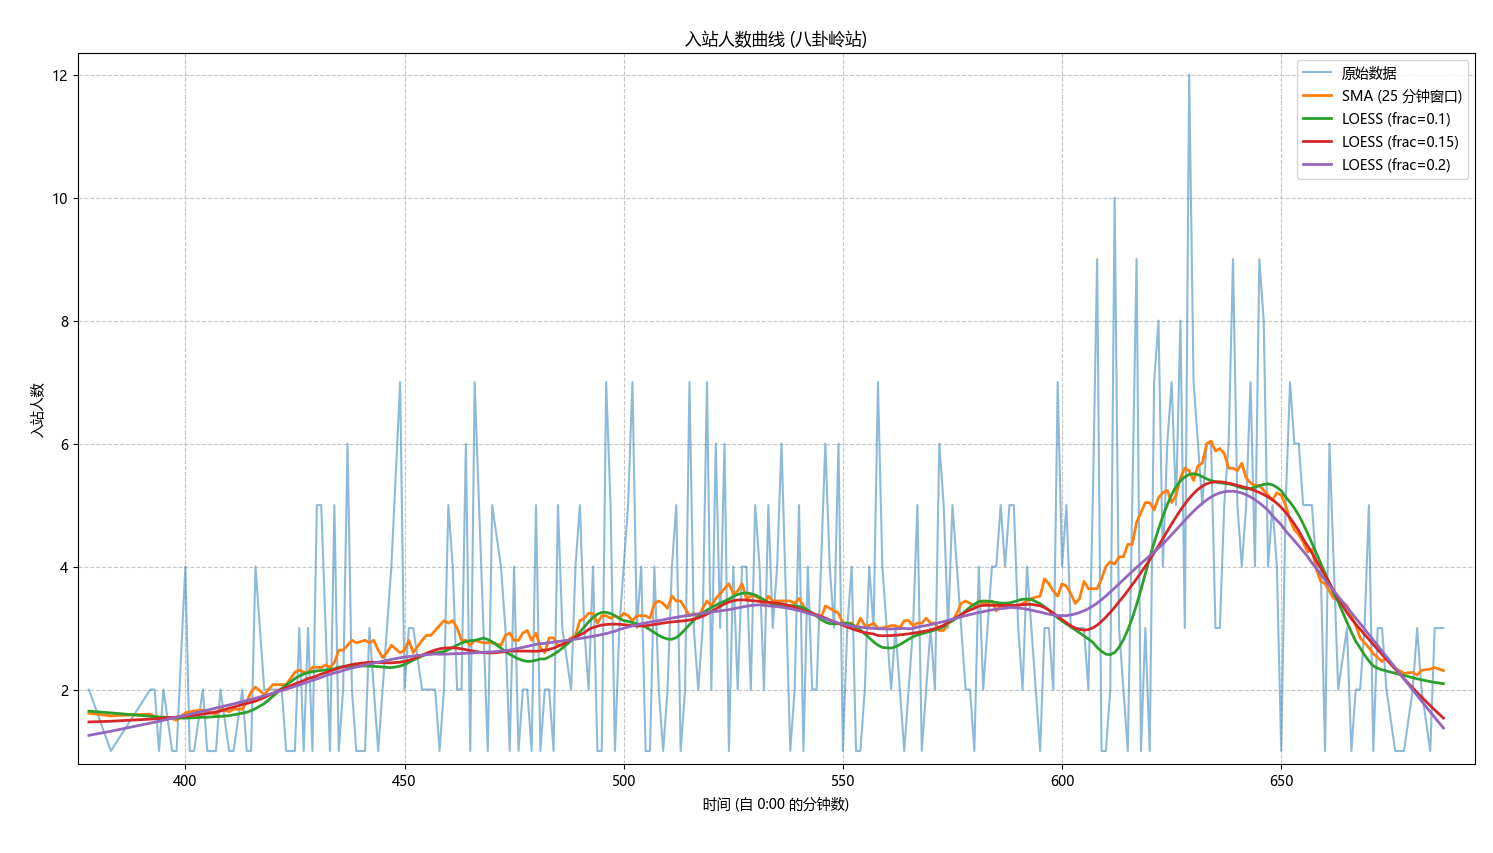
\includegraphics[width=1.0\textwidth]{res/Figure_2.png}
    \label{fig:entryCurveBagualing}
\end{figure}

\begin{figure}[htbp]
    \centering
    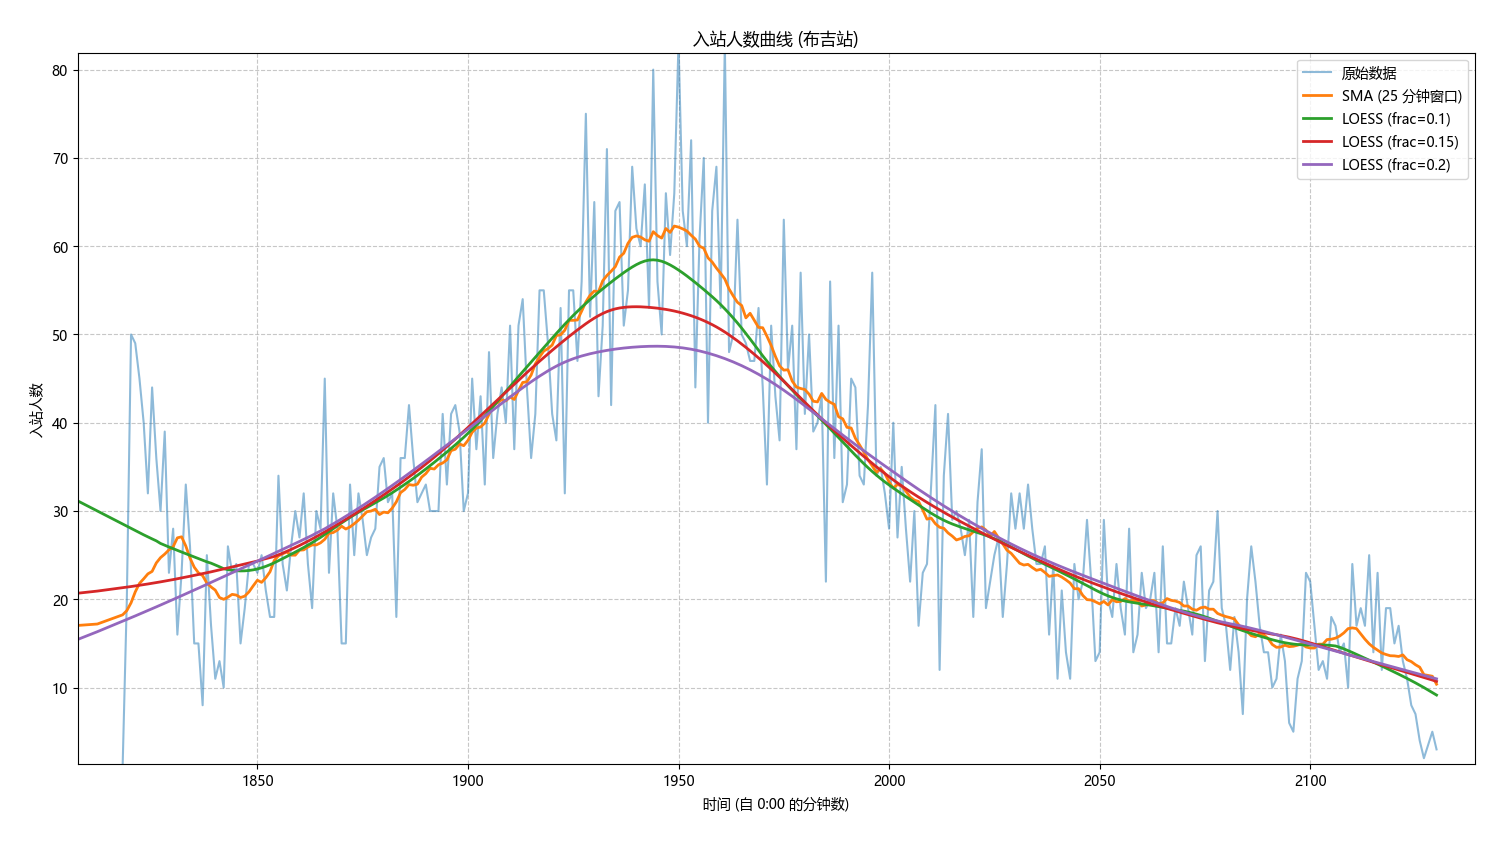
\includegraphics[width=1.0\textwidth]{res/Figure_3.png}
    \label{fig:entryCurveBuji}
\end{figure}

同时,考察八卦岭站(图 \ref{fig:entryCurveBagualing})和布吉站(图 \ref{fig:entryCurveBuji}),会发现各站点高峰时间、高峰客流模式均存在差异。
为了平衡曲线的平滑度和对主要高峰特征的捕捉能力,经初步实验,选定 frac=0.2 的 LOESS 算法作为平滑化处理。

$$
L_i(t) = \text{LOESS}(E_i, frac=0.2)(t)
$$

不同站点的客流高峰时间、形态存在差异,为了构建一个适用于一般性分析或作为基准的平均模式,我们采用动态时间规整(DTW)\cite{DTW}技术,将各站点的平滑曲线 $L_i(t)$ 在时间轴上向一个参考站点,此处以五和站为例。

然后选定五和站为标准进行 DTW 规整。值得注意的是,在 DTW 对齐过程中,我们发现如果直接使用原始数据进行对齐,容易出现对齐后曲线与标准数据曲线高度重合、高峰部分则异变为水平直线(最大值和研究数据相同)的现象。
我们推测这是因为研究数据与标准数据的局部波动(如小峰值或噪声)不一致,DTW 会在这些区域频繁调整路径,导致对齐后的时间轴不平滑。
因此,我们使用 min-max 归一化后的数据作为 DTW 参数,这是很有效的。

$$
N_i(t) = \frac{L_i(t) - \min_{t'}L_i(t')}{\max_{t'}L_i(t') - \min_{t'}L_i(t')}
$$

$$
P_i(t) = \text{DTW\_Align}(L_i, N_i, N_{ref})(t)
$$

我们将所有站点经过 DTW 对齐后的客流曲线 $P_i(t)$ 进行平均,得到一个代表性的平均客流到达模式 $\bar{P}(t)$。

\begin{figure}[htbp]
    \centering
    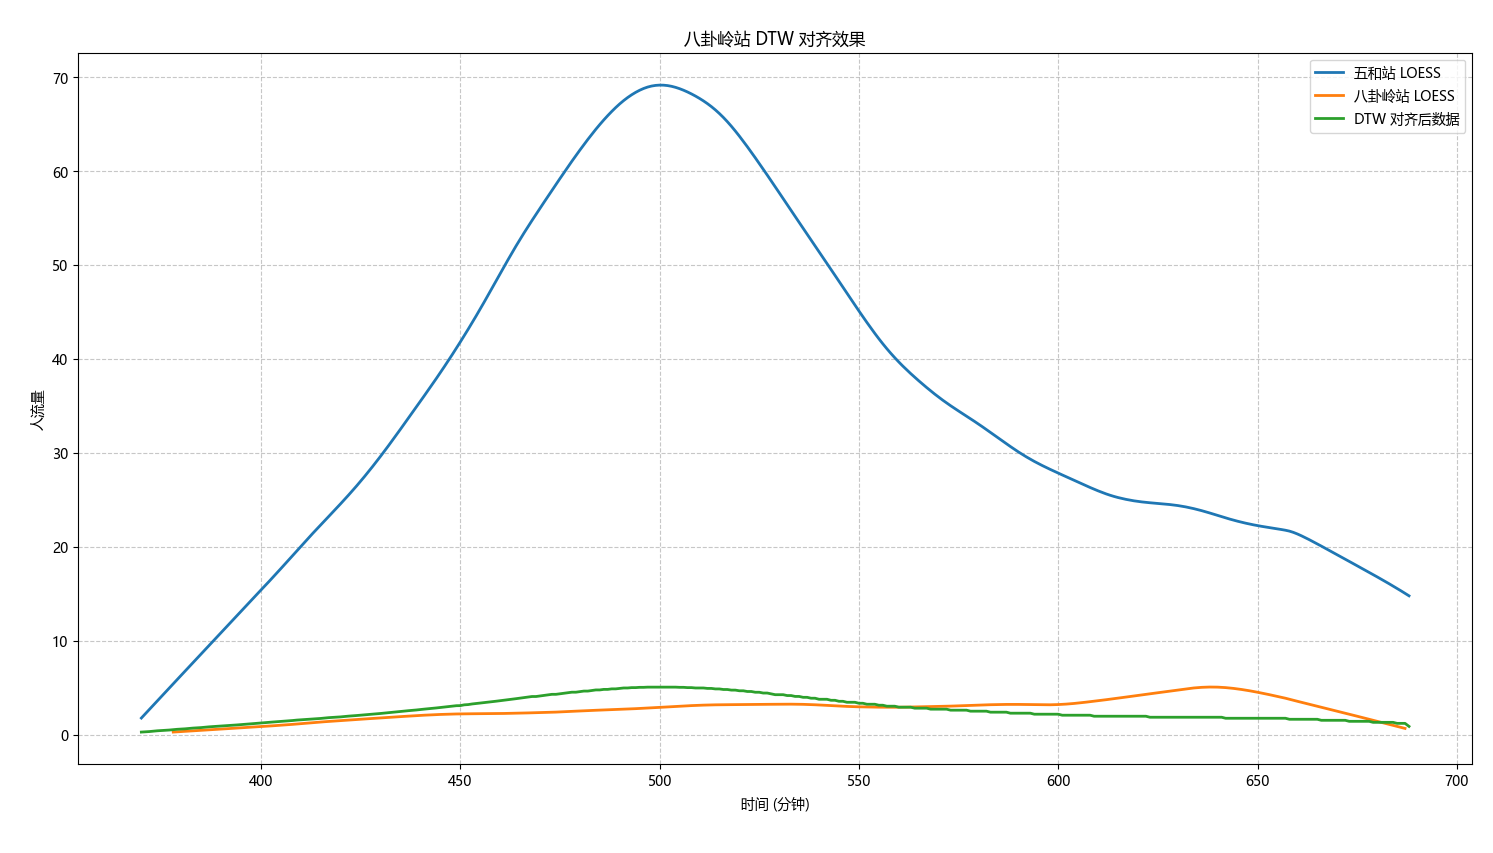
\includegraphics[width=1.0\textwidth]{res/Figure_5.png}
    \label{fig:alignedBagualing}
\end{figure}

八卦岭站的高峰时间相对于五和站(我们选择的参考站点)较晚,数据中客流量小。如图 \ref{fig:alignedBagualing} 所示,DTW 算法较好地规整了这一时间差异。

$$
\bar{P}(t) = \frac{1}{n} \sum_{i} P_i(t)
$$

我们将这个经验平均曲线 $\bar{P}(t)$ 作为未来时段(0:00-12:00)的预测乘客到达速率函数,即 $P(t) = \bar{P}(t)$。这个 $P(t)$ 函数直接反映了历史数据的平均模式,避免了拟合特定数学公式可能带来的模型设定偏差。

\mcmSubsection{问题二:站点对模型进行还原}

还是需要再次强调,我们在前述研究中使用多站点的单天数据,是因为我们只能获取到这些数据。实际使用中,站点可以使用自己的历史数据,进一步地实现个性化和实时修正。大致思路如下:
\begin{enumerate}
    \item \textbf{基准模型:} 使用历史多日数据(而非多站点单日数据)为特定站点 $i$ 计算其自身的基准到达率函数 $P_{base, i}(t)$。
    \item \textbf{实时数据收集:} 在运营当天,收集截至当前时刻 $t_{now}$ 的实际入站数据 $E_{real}(t)$ for $t \in [0, t_{now}]$。
    \item \textbf{模型修正:} 使用 $E_{real}(t)$ 与 $P_{base, i}(t)$ 在 $[0, t_{now}]$ 区间的数据,通过 DTW 调整 $P_{base, i}(t)$ 在未来时段 $[t_{now}, T_{op}]$ 的预测值,得到实时修正后的预测 $P_{current}(t)$。
    \item \textbf{滚动优化:} 使用 $P_{current}(t)$ 重新运行后续的优化算法,动态调整发车计划。
\end{enumerate}
这部分是模型应用的重要扩展,使得模型具有适配各个站点实际情况的实用价值。

\mcmSubsection{问题三:发车时刻优化}

我们采用遗传算法(GA)\cite{HollandGA}来优化 0:00 至 12:00($T_{op}=720$ 分钟)期间的发车时刻表。为了允许模型自我调整,只求解下一次发车的时间,而不是完整的时刻表。\cite{GoldbergGA}

优化目标是最小化单位时间内成本,包括发车次数成本和乘客等待时间成本。

$$
\text{Cost}(t) = \frac{\gamma \int _0 ^T P(\tau)(T-\tau)d\tau + \eta}{T}
$$

为了综合考虑乘客体验和运营成本,经过多次测试,选定 $\gamma=2.0$ 和 $eta=10.0$ 作为参数。设计如下的遗传算法:

\begin{enumerate}
    \item 个体:发车间隔 $T$,取值范围为 $[T_{\min}, T_{\max}]$
    \item 适应度函数:计算每个 $T$ 对应的目标函数值 $\text{Cost}(T)$ 的倒数
    \item 初始化种群:在取值范围内随机生成个体
    \item 选择操作:轮盘赌
    \item 交叉操作:加权平均父代基因
    \item 变异操作:添加高斯噪声,同时确保在取值范围内
    \item 终止条件:达到最大迭代次数或适应度收敛
\end{enumerate}

最终,适应度最高的个体代表了下一次发车的最优(近优)时间。

如图 \ref{fig:gaBuji1} 所示,高峰期时(距离 0:00 50 分钟),模型建议 4.95 分钟后发车;在高峰后客流逐渐减少的 600 分钟时,模型则建议 6.01 分钟后发车。

\begin{figure}[htbp]
    \centering
    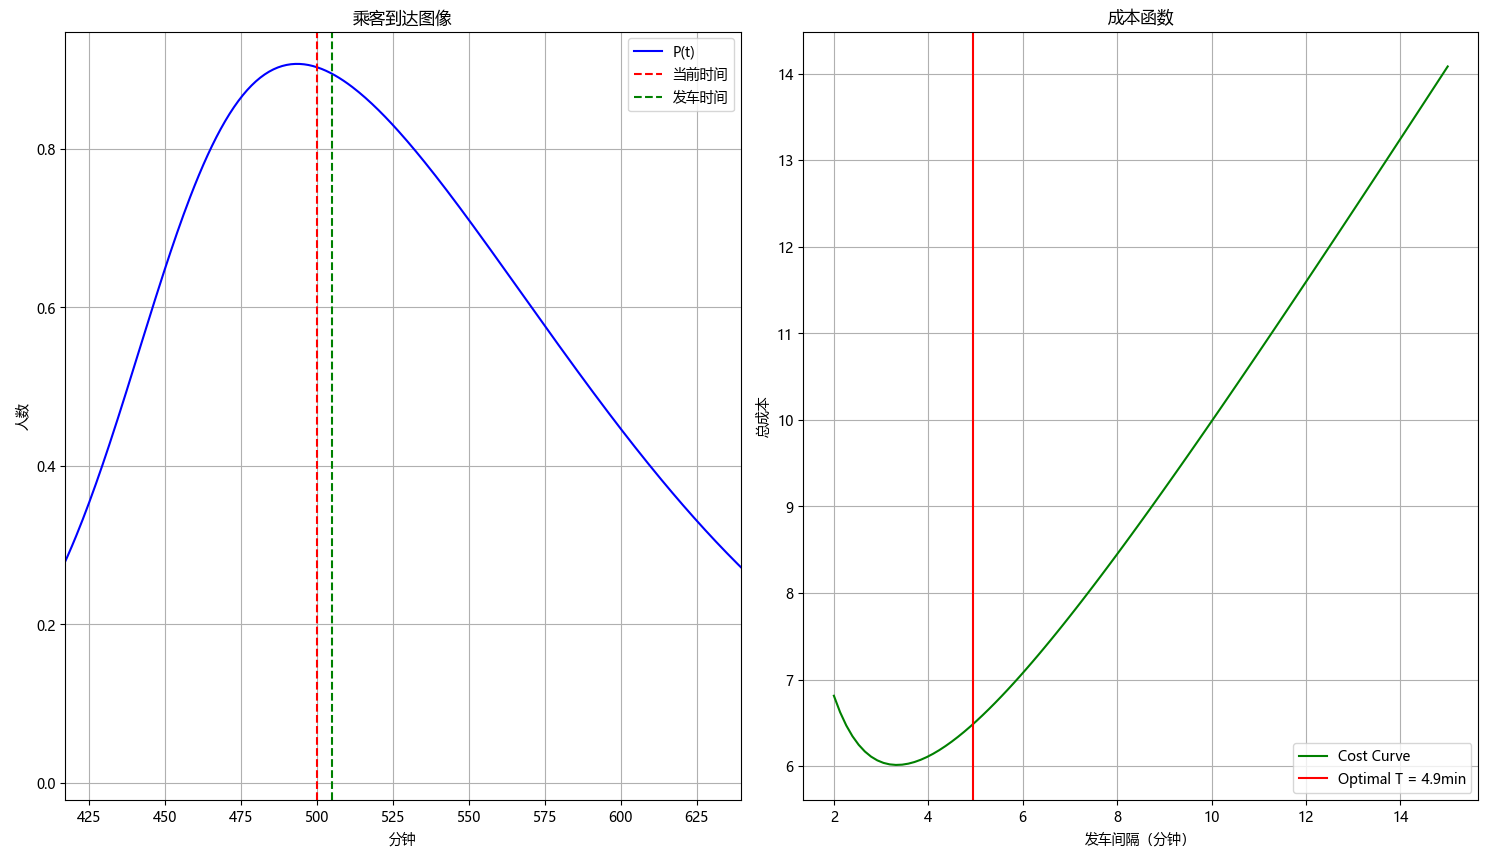
\includegraphics[width=1.0\textwidth]{res/Figure_7.png}
    \label{fig:gaBuji1}
\end{figure}

\begin{figure}[htbp]
    \centering
    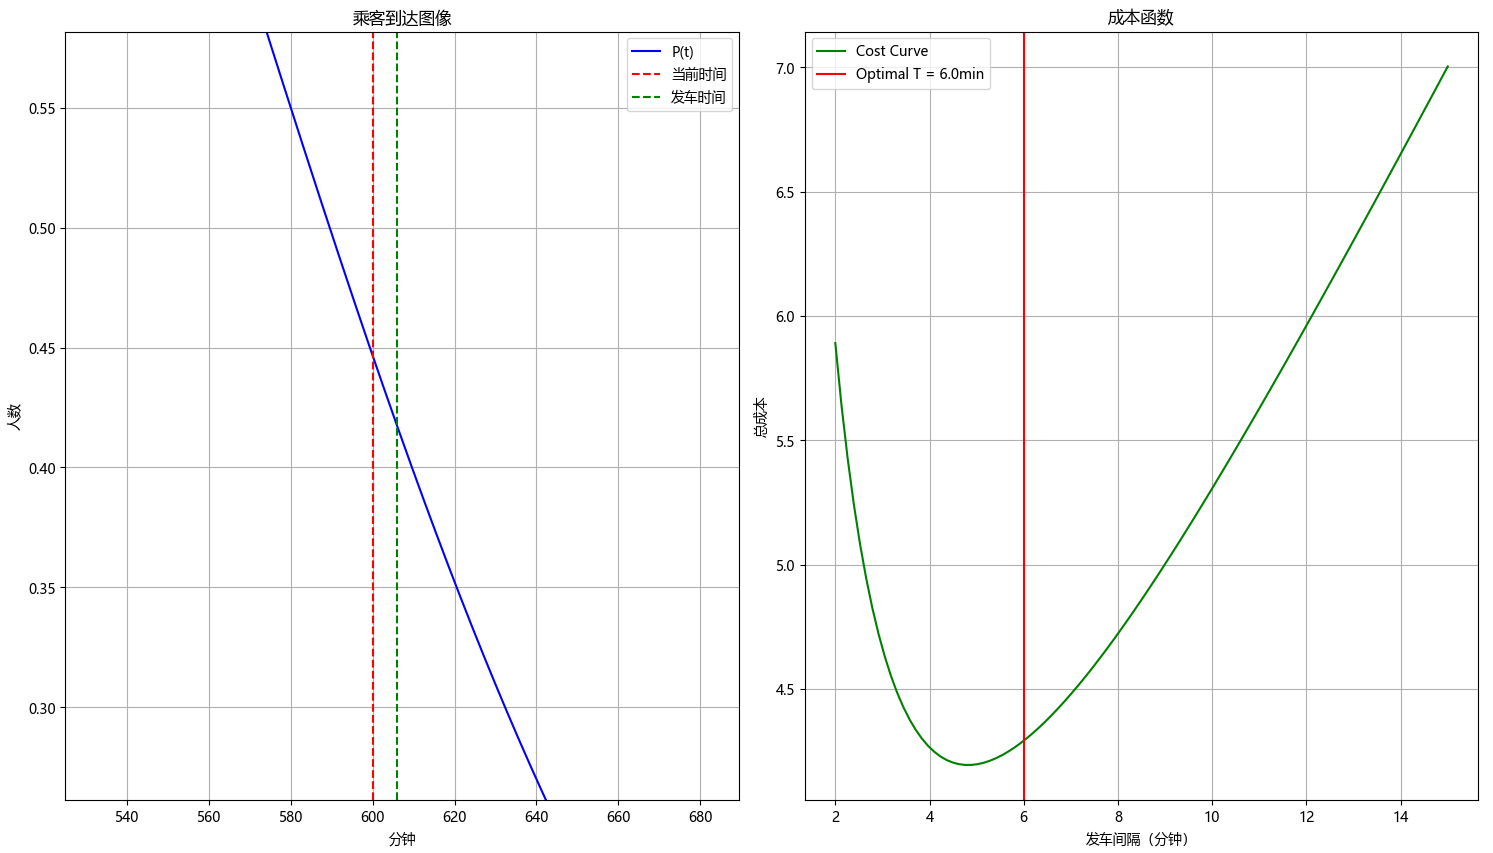
\includegraphics[width=1.0\textwidth]{res/Figure_8.png}
    \label{fig:gaBuji2}
\end{figure}

\mcmSection{模型的评价与改进}

\begin{enumerate}
    \item \textbf{优点:}
        \begin{itemize}
            \item \textbf{适应性:} 模型基于历史客流数据构建预测 $P(t)$,并通过仿真优化,能够适应客流的时间波动性,相比固定间隔更有效率。
            \item \textbf{理论基础:} 采用基于仿真的优化,直接模拟了排队、登车和容量限制过程,比仅基于简单公式的成本函数更贴近现实物理过程。优化目标明确(总等待时间 vs 发车次数)。
            \item \textbf{多目标:} 通过调整权重 $\gamma, \eta$,可以在乘客服务水平和运营成本之间进行权衡,为决策者提供不同策略下的方案。
            \item \textbf{自动化:} 整个流程(数据处理、预测、仿真、优化)可以自动化执行,减少人工排班的复杂性。
            \item \textbf{可扩展性:} 步骤二中描述的实时修正框架,为模型对接实时数据、实现动态调度提供了基础。
        \end{itemize}
    \item \textbf{缺点:}
        \begin{itemize}
            \item \textbf{依赖预测:} 优化结果的有效性高度依赖于客流预测 $P(t)$ 的准确性。历史平均可能无法捕捉突发事件或特殊日期的客流变化。
            \item \textbf{仅适用单站点优化:} 本研究未考虑线路协调。单个站点的最优发车计划可能与线路上其他站点的需求或约束冲突。考虑到已有其他研究建立了模型调解这样的冲突,故本研究忽略了这一点。
            \item \textbf{参数敏感性:} 模型性能对某些参数(GA 参数、成本权重 $\gamma, \eta$)的选择比较敏感,需要仔细调试和标定。
            \item \textbf{GA收敛性:} 遗传算法提供的是近优解,不保证全局最优。结果可能受初始种群、算子设计的影响,需要多次运行或精调参数以获得稳定可靠的解。
        \end{itemize}
\end{enumerate}

\textbf{改进方向}

基于上述评价,未来可以从以下几个方面对模型进行改进:
\begin{enumerate}
    \item \textbf{提升客流预测精度:}
        \begin{itemize}
            \item 采用更先进的时间序列预测模型(如 SARIMA, Prophet, LSTM 等神经网络模型)替代当前的经验平均法,以更好地捕捉季节性、趋势和潜在的非线性模式。
            \item 融合多源数据,如天气信息、节假日安排、周边活动事件等,提高预测对异常情况的适应能力。
        \end{itemize}
    \item \textbf{细化仿真模型:}
        \begin{itemize}
            \item 在仿真中更精确地模拟乘客行为,如考虑乘客因拥挤或等待时间过长而放弃乘坐的可能性。
            \item 引入更详细的站台物理模型,考虑站台拥挤度对乘客移动速度、上下车效率的影响。
            \item 区分不同类型乘客(如通勤、休闲、携带大件行李者)可能存在的不同行为模式。
            \item 考虑列车实际到站时间的不确定性,而非假设完全按计划时刻到达。
        \end{itemize}
    \item \textbf{引入鲁棒性和随机性考量:}
        \begin{itemize}
            \item 明确处理客流预测的不确定性:使用概率性预测(给出预测区间而非单点预测值),优化目标可以变为最小化期望成本或在一定置信水平下的最差情况成本。
            \item 在仿真中使用随机到达过程代替确定性的到达率函数 $P(t)$,使评估更接近实际运营中的随机波动。
            \item 优化算法可以考虑随机环境下的性能,例如采用随机模拟优化方法。
        \end{itemize}
    \item \textbf{实证验证与标定:}
        \begin{itemize}
            \item 使用更广泛、时间跨度更长的真实地铁运营数据(包括客流、实际发车时刻、列车满载率等)来验证模型的预测精度和优化效果。
            \item 与地铁运营部门合作,进行参数标定(特别是成本系数 $\gamma, \eta$),使其更符合实际运营目标和约束。
            \item 如果可能,进行小范围试点应用,比较模型生成的时刻表与现有时刻表在实际运营中的表现。
        \end{itemize}
\end{enumerate}

\mcmSection{结论}

本研究针对城市轨道交通系统中固定发车间隔模式在应对客流波动方面的局限性,提出了一种基于历史客流数据和仿真优化的单站点动态发车时刻表生成方法。通过对深圳通刷卡数据的预处理,我们构建了一个能够反映代表性日客流模式的预测乘客到达速率函数 $P(t)$。

核心创新在于采用基于仿真的遗传算法(GA)进行优化。GA 的适应度函数通过模拟站台的排队过程来评估,综合考虑了列车容量限制、乘客总等待时间。通过调整权重系数 $\gamma$ 和 $\eta$,该模型能够在最小化乘客等待成本和降低运营成本这两个目标之间进行权衡。

模型预期结果表明,优化后的发车时刻表呈现动态特性:在预测的客流高峰时段,发车间隔缩短,以快速疏散乘客、降低等待时间;在平峰时段,发车间隔则相应延长,以避免资源浪费、节约运营成本。这种数据驱动的动态调度策略,相比传统的固定间隔模式,有望显著提升乘客出行体验和地铁系统运营效率。

尽管本研究存在一些简化假设且优化效果依赖于客流预测的准确性,但所提出的框架——结合数据处理、客流预测、仿真评估和智能优化算法——为实现更精细化、更具适应性的地铁运营调度提供了有价值的思路和方法论基础。未来的工作可集中于提升预测精度、考虑线路网络协调、细化仿真模型以及进行更广泛的实证验证,从而将该方法推向实际应用,助力智慧城市交通系统的发展。